\chapter{Mathematical Formulation}
\label{mathchapter}

The objective of this fake thesis document is to demonstrate
a multitude of \LaTeX{} features as well as features specific
to the thesis class.
We start by giving one short formula,
and one big hairy multi-line formula
(one of the non-dimensional Navier-Stokes equations):

\begin{equation}
	A = \pi r^2
\end{equation}


\begin{eqnarray}
  \rho \left[ \frac{DV_r}{Dt} - M \epsilon^2
    \frac{\vth^2}{r} \right]
  & = & -\frac{\delta^2}{\gamma~ M} \diffr{P}
	+ \frac{M ~\delta^2}{Re} \left\{ 2 \diffr{}
	\left[ \mu \left( \diffr{V_r}
        - \frac{1}{3} {\bf \nabla \cdot \overline{V}}
      \right) \right] \right. \nonumber \\
  & & + \frac{1}{r} \diffth{} \left[ \mu \left(
      \frac{1}{r} \diffth{V_r} + \epsilon \diffr{\vth}
      - \epsilon \frac{\vth}{r} \right) \right] \nonumber \\
  & & + \diffz{} \left[ \mu \left( \frac{1}{\delta^2}
        \diffz{V_r} + \diffr{V_z} \right) \right] \nonumber \\
  & & + 2 \left. \frac{\mu}{r}\left[ \diffr{V_r} -\frac{\epsilon}{r}
      \diffth{\vth} - \frac{V_r}r\right] \right\}, \label{eq:rmom}
\end{eqnarray}


\section{Explanation of equations}

The latter equation is non-dimensionalized using the following definitions:

\[
	r = \frac{r'}{R'}, ~~~
	z = \frac{z'}{L'},~~~
	t = \frac{t'}{t_a'}, ~~~
	\kappa = \frac{\kappa'}{\kappa_0'}, ~~~
	\mu = \frac{\mu'}{\mu_0'} , ~~~
	C_V = \frac{C_V'}{C_{V0}'},
\]
where $P_0'$ is the initial static pressure in the cylinder,
and $\rho_0'$ and $T_0'$ are the density and temperature
of the fluid being injected from the sidewall.

\begin{figure}[htbp]
    \caption[Cutting up a triangular pyramid]{
	A triangular pyramid may be cut up as shown, to
	yield one top pyramid (with one-eighth the volume
	of the full pyramid), three bottom corner pyramids
	(which, when joined, are congruent to the top pyramid),
	three prisms along the bottom edges (the area of whose
	bottom faces total $B/2$) and the large central prism
	(volume = $(B/4)(h/2) = Bh/8$).
	The image, from PDF file ``pyr.pdf'',
	was read in using the {\tt $\backslash$includegraphics}
	command, from the {\tt graphicx} package.
	}
    \begin{center}
	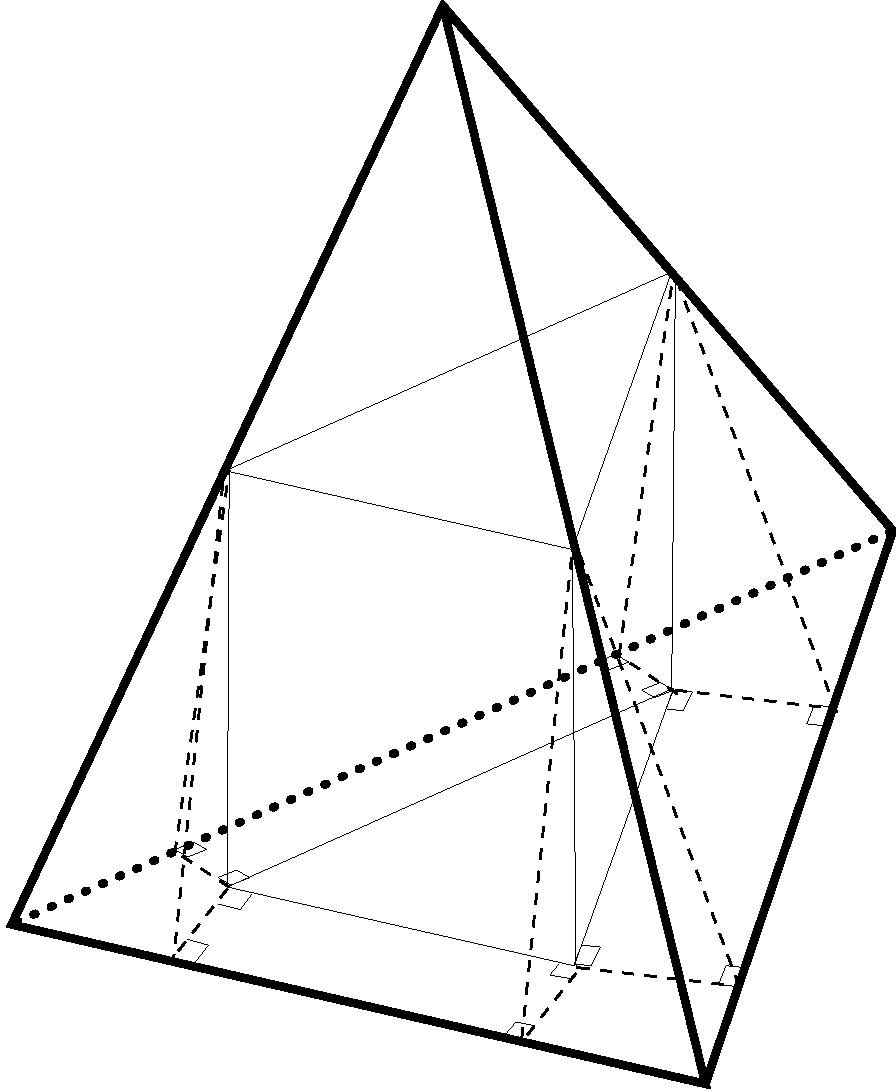
\includegraphics[width=90mm]{figs/pyr.pdf}
    \end{center}
\label{pyramid}
\end{figure}


Here is an example of using the macros
\verb2\singlespacing2 and \verb2\doublespacing2:

\singlespacing	% <------------------------------

This paragraph was preceded by the
command \verb2\singlespacing2.
See the Specifications of the Grad School for instructions
about when single spacing is appropriate in a thesis.

\doublespacing	% <------------------------------

And now, here is an example of using the macros
\verb2\begin{singlespace}2 and \verb2\end{singlespace}2;
another way to get single-spacing.

\begin{singlespace}	% <-----------------------------
Two cases are studied in the present work which differ only in the
boundary conditions.  Each different boundary condition model a
different source of instability.  The boundary of the first case
consists of a steady, axisymmetric sidewall radial velocity boundary
and a time-dependent, non-axisymmetric endwall axial velocity
boundary.  The second case is studied with a fixed impermeable axial
velocity along the endwall and a combination axisymmetric steady and
non-axisymmetric unsteady radial velocity along the sidewall.
\end{singlespace}	% <-----------------------------


Usually you want to use a table produced by some other
software, such as Excel, rather than try to do it using
\LaTeX macros.  If the table is saved/printed to a PDF file,
then it can be displayed using the
$\backslash${\tt includegraphics} macro
inside a {\tt table} environment:


\begin{table}
    \caption[Table from a PDF file]{
	This table wasn't constructed with \LaTeX{}
	commands, but resides in PDF file
	({\tt tableD.pdf})
	created by some other software.
	}
    \begin{center}
	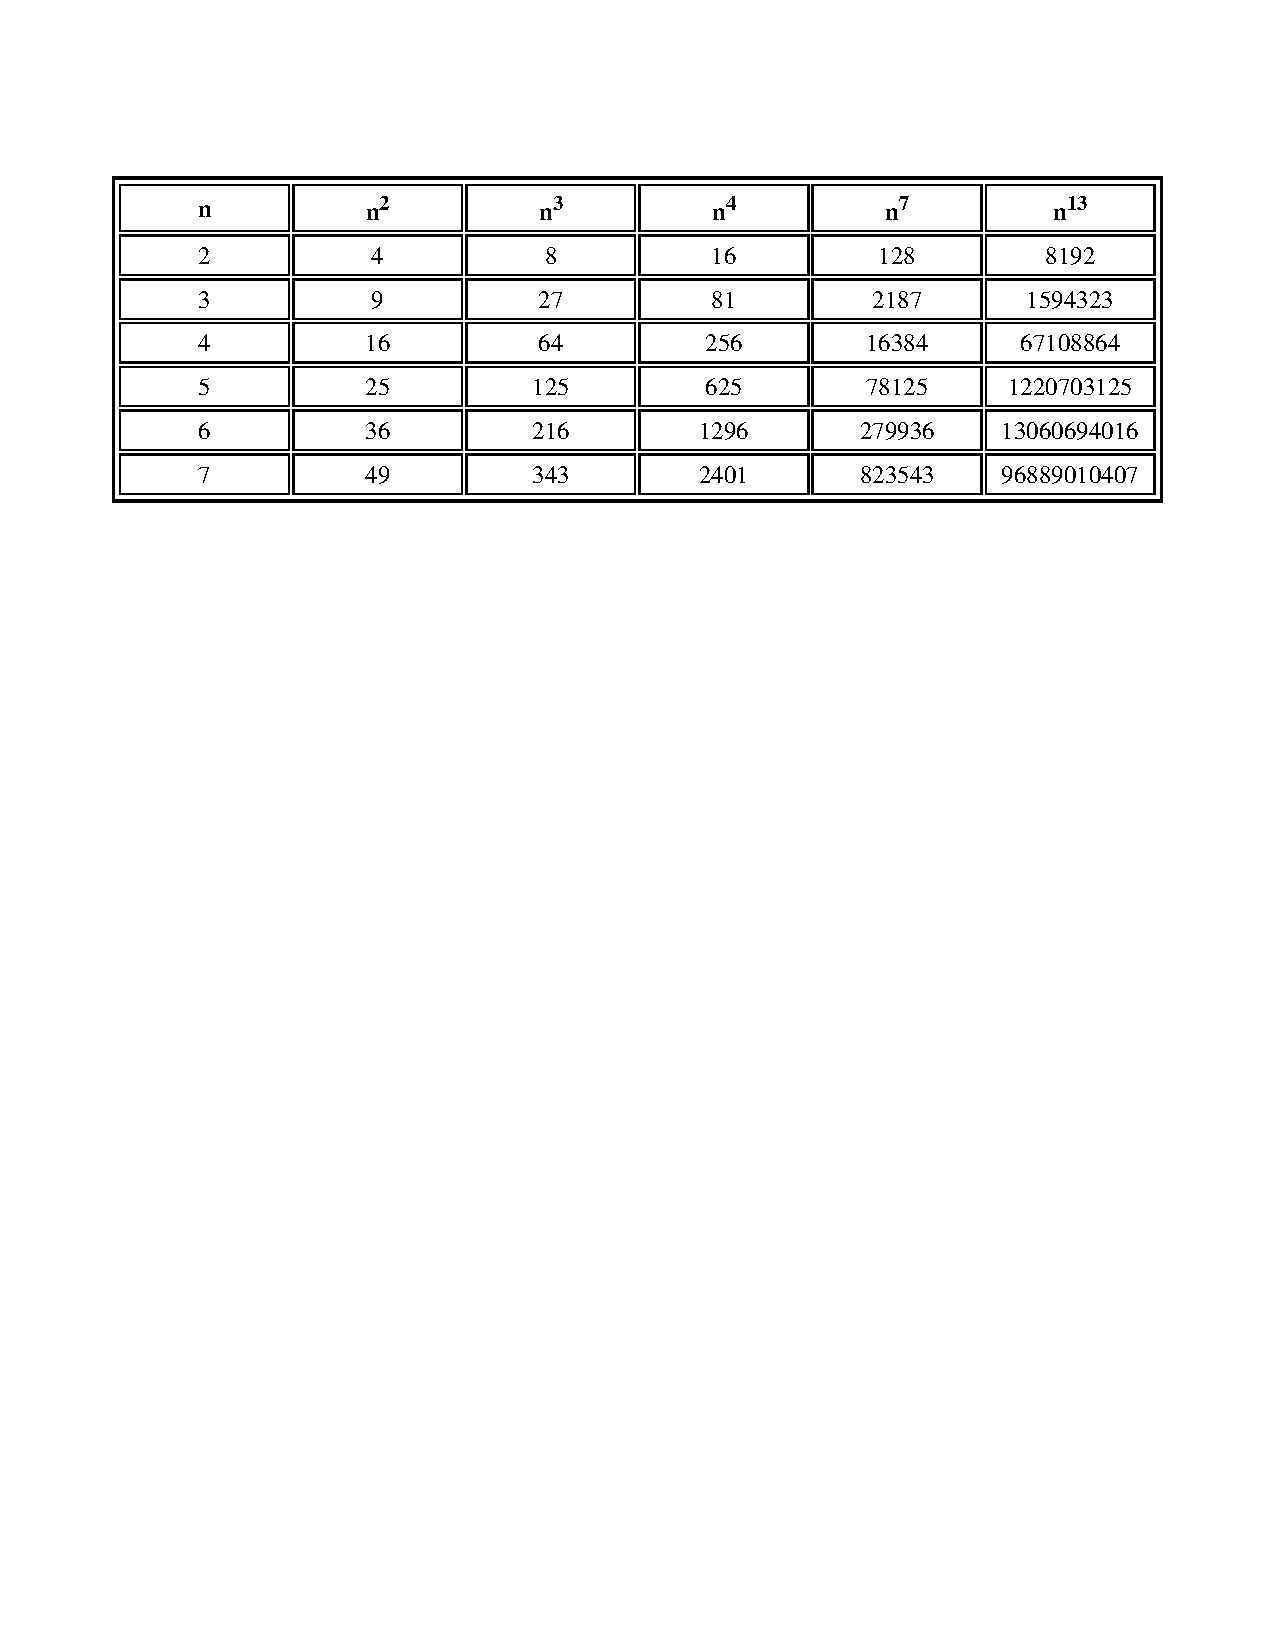
\includegraphics[width=5.45in]{figs/tableD.pdf}
    \end{center}
\label{pdftable}
\end{table}


Some of the boundary conditions are:

\begin{eqnarray}
  z=0; && V_z = \twochoices
	{0, && t\leq0}
	{\widetilde{F}_{zw}(r,\theta,t), && t>0}
						\label{eq:endwall} \\
  z=0; && V_{\theta}=V_r=0			\label{eq:endnoslip} \\
  r=0; && P,\rho,T,V_r,\vth,V_z~\mbox{finite},	\label{eq:centerline} \\
  r=1; && V_r= F_{rws}(z),			\label{eq:injection} \\
  r=1; && V_z=\vth =0,				\label{eq:sidenoslip}
\end{eqnarray}
and solutions must be periodic in $\theta$.

If you don't believe this stuff, check out
Mulick\cite{mulick} and Baylor\cite{baylor}.


\section{Yet another section}

\subsection{
	Just meaningless text to test lines per page
	\label{ss}}

According to the Grad School specs.   there should be 24--27 lines
of print per page of a thesis.  This should be true whether the font
size is 10, 11, or 12.  Count them up; does this document conform?
According to the Grad School specs.   there should be 24--27 lines
of print per page of a thesis.  This should be true whether the font
size is 10, 11, or 12.  Count them up; does this document conform?
According to the Grad School specs.   there should be 24--27 lines
of print per page of a thesis.  This should be true whether the font
size is 10, 11, or 12.  Count them up; does this document conform?
According to the Grad School specs.   there should be 24--27 lines
of print per page of a thesis.  This should be true whether the font
size is 10, 11, or 12.  Count them up; does this document conform?
According to the Grad School specs.   there should be 24--27 lines
of print per page of a thesis.  This should be true whether the font
size is 10, 11, or 12.  Count them up; does this document conform?
According to the Grad School specs.   there should be 24--27 lines
of print per page of a thesis.  This should be true whether the font
size is 10, 11, or 12.  Count them up; does this document conform?
According to the Grad School specs.   there should be 24--27 lines
of print per page of a thesis.  This should be true whether the font
size is 10, 11, or 12.  Count them up; does this document conform?
According to the Grad School specs.   there should be 24--27 lines
of print per page of a thesis.  This should be true whether the font
size is 10, 11, or 12.  Count them up; does this document conform?
According to the Grad School specs.   there should be 24--27 lines
of print per page of a thesis.  This should be true whether the font
size is 10, 11, or 12.  Count them up; does this document conform?
According to the Grad School specs.   there should be 24--27 lines
of print per page of a thesis.  This should be true whether the font
size is 10, 11, or 12.  Count them up; does this document conform?
According to the Grad School specs.   there should be 24--27 lines
of print per page of a thesis.  This should be true whether the font
size is 10, 11, or 12.  Count them up; does this document conform?
According to the Grad School specs.   there should be 24--27 lines
of print per page of a thesis.  This should be true whether the font
size is 10, 11, or 12.  Count them up; does this document conform?
According to the Grad School specs.   there should be 24--27 lines
of print per page of a thesis.  This should be true whether the font
size is 10, 11, or 12.  Count them up; does this document conform?
According to the Grad School specs.   there should be 24--27 lines
of print per page of a thesis.  This should be true whether the font
size is 10, 11, or 12.  Count them up; does this document conform?
According to the Grad School specs.   there should be 24--27 lines
of print per page of a thesis.  This should be true whether the font
size is 10, 11, or 12.  Count them up; does this document conform?
According to the Grad School specs.   there should be 24--27 lines
of print per page of a thesis.  This should be true whether the font
size is 10, 11, or 12.  Count them up; does this document conform?
According to the Grad School specs.   there should be 24--27 lines
of print per page of a thesis.  This should be true whether the font
size is 10, 11, or 12.  Count them up; does this document conform?

\paragraph{What is it?}
This is a labelled paragraph.
The heading of the paragraph is emphasized.
This is a labelled paragraph.
The heading of the paragraph is emphasized.

\subsection{This is a subsection}

This is a subsection.
Filler filler filler filler filler filler filler filler.
Filler filler filler filler filler filler filler filler.

\subsection{This is another subsection}

This is another subsection.
Filler filler filler filler filler filler filler filler.
Filler filler filler filler filler filler filler filler.

\paragraph{This is paragraph number 2.}
It used a \verb2\paragraph{}2 header, which
are always inlined (with extra space)
and  boldfaced.

This is the third paragraph of the subsection.
Filler filler filler filler filler filler filler filler.
Filler filler filler filler filler filler filler filler.

%%%%%%%%%%%%%%%%%%%%%%%%%%%%%%%%%%%%%%%%%%%%%%%%%%%%%%%%%%

\subsubsection{This is a subsubsection (1)}
This is the first paragraph of the subsubsection.
Whether it is numbered or inlined depends on the
option selected at the beginning of the
thesis.

By default, a \verb2\subsubsection2 heading is numbered
and set off on a separate line, left-justified.

\paragraph{However.}
Using the \verb2inlineh42 option, subsubsection headers
are inlined.
And using the \verb2nonumh42 option suppresses
numbering of the subsubsections.
Together they make subsubsection headings
just the same as paragraph headings.


%%%%%%%%%%%%%%%%%%%%%%%%%%%%%%%%%%%%%%%%%%%%%%%%%%%%%%%%%%

\subsubsection{
	This is another subsubsection (2)
	\label{sss}
	}

Once again, whether its heading is numbered
and/or inlined depends on the class options
chosen at the start.

There is no ``subsubsubsection'' entity,
and ``subparagraph'' gets no special treatment
in \emph{thesis} class.

\section{The End}
\label{sec:end}

Finally, this is the end.  The bibliography starts on
the next page.
Note how the \verb2\hyperref2 package
(mentioned in chapter \ref{introchap})
also makes hyperlinks from references
(e.g., Mulick\cite{mulick})
to entries in the bibliography.

